%!TEX root = ../doc.tex
\chapter{Industrie Demonstrator}
\label{sec:montageaufgabe}
In der Bachelorarbeit von Andrin Meister und Christian Hartmann wurde ein Grossteil des Aufbaus und der Funktionalitäten des Industrie 4.0 Demonstrators definiert. In den folgenden Abschnitten wird kurz auf die für den Montageprozess mit dem Sechsachsroboter der Firma Stäubli wichtigsten Punkte eingegangen. 

\section{Physikalische Schnittstellen}\label{sec:HWSchnittstellen}
Der Industrie Demonstrator ist modular Aufgebaut, es gibt 3 trennbare Module, die Montagezelle mit dem Industrieroboter befindet sich in der mittleren Zelle. Der Arbeitsraum des Roboters ist nahezu nicht durch andere Systeme im Demonstrator beschränkt. Die einzigen physikalischen Interaktionen mit dem gesamt System bestehen aus dem Greifen der Teile aus den Teileträgern, welche auf Linearschlitten montiert sind. Auch im Mittelteil der Anlage wird ein Portalroboter verbaut, welcher sich in der Nähe des Sechsachsroboters bewegt. 
\begin{figure}[h!]
	\centering
	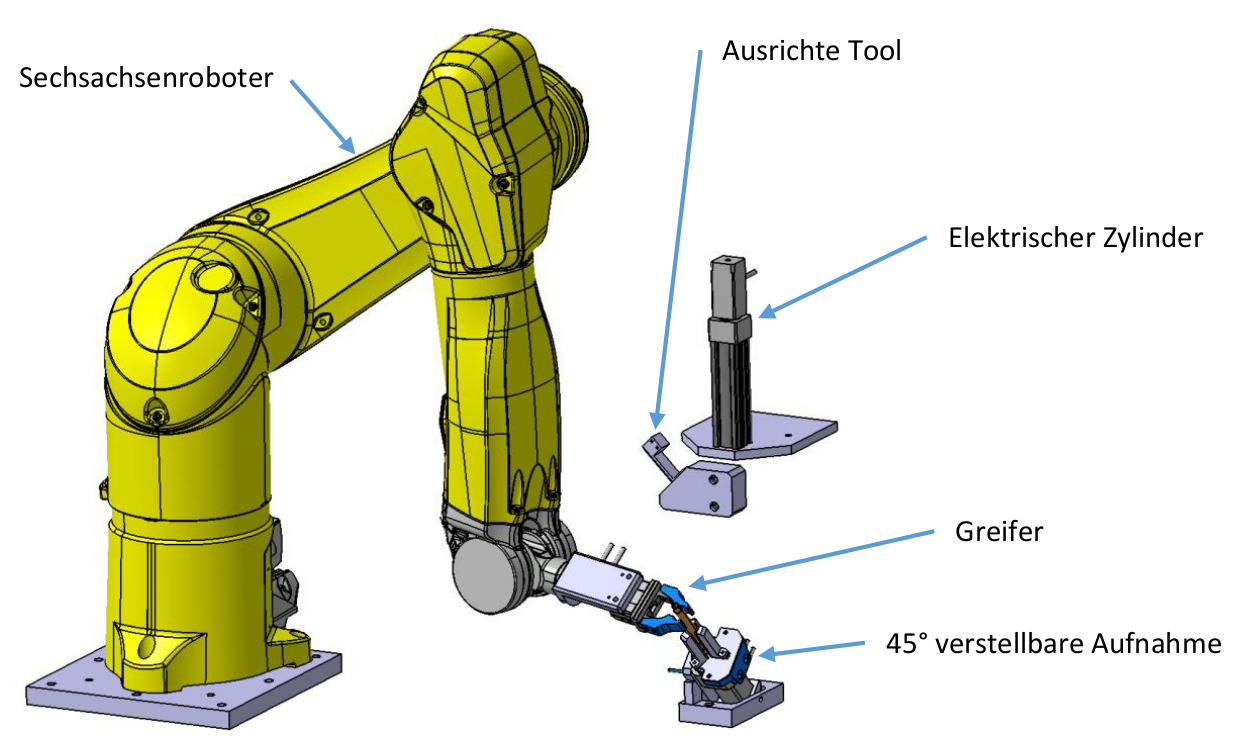
\includegraphics[width=0.8\textwidth]{workcell}
	\caption[Hauptelemente der Montagestation]{Hauptelemente der Montagestation\cite{Hartmann2017}}
	\label{fig:workcell}
\end{figure}

\section{Software Schnittstellen}\label{sec:SWschnittstellen}
Der Grossteil der Anlage wird über Siemens SPS Steuerungen angesteuert, welche über PROFINET kommunizieren. Eine Einbindung dieses Protokolls in eine Linux/ROS Umgebung ist sehr komplex. Aus diesem Grund wurde mit den restlichen am Industrie 4.0 Demonstrator beteiligten Personen definiert, dass der der Linux PC gegen Aussen ein Webserver zur Verfügung stellt. Der zentralen Steuerung der Anlage soll es dabei möglich sein, einen Montagevorgang auszulösen sowie den Status des Roboters abzufragen. \\
Von ROS aus muss zudem die Ansteuerung des Dreibackengreifers, der Presse, sowie des Greifers am Roboterarm geschehen. Bei all diesen Aktuatoren handelt es sich um Servomotoren der Firma SMC welche mit Controllern mit einem EtherCAT Interface angesteuert werden können.

\section{Kugelschreibermontage}
Der Kugelschreiber, welcher zusammengebaut werden soll, besteht aus insgesamt aus fünf Teilen. Diese Einzelteile liegen definiert im Schlitten des Transportsystems, welche an einer vordefinierten Stelle im Arbeitsbereich des Roboters anhalten. Diese Teileträger befinden sich während des ganzen Montageprozesses an der selben Position.
Der Montageablauf besteht aus folgenden Schritten:
\begin{enumerate}
	\item Vorderhülle in Dreibackengreifer positionieren
	\item Vorderhülle mithilfe des ausrichte Tools in korrekte Position drehen
	\item Feder in Vorderhülle einführen
	\item Miene in Vorderhülle einführen
	\item Arretierung aufsetzen
	\item Dreibackengreifer inkl. Kugelschreiber in senkrechte Lage drehen
	\item Deckel positionieren und aufpressen
	\item Dreibackengreifer inkl. Kugelschreiber in 45\textdegree Lage drehen
	\item Kugelschreiber entnehmen
\end{enumerate}
Der Grundsätzliche Ablauf für die Montage des Kugelschreibers ist durch die Geometrie des Kugelschreibers gegeben, wie genau diese Teile gegriffen werden und wie die Montagestation aufgebaut ist wurde in der Bachelorarbeit von Andrin Meister und Christian Hartmann definiert und sind somit für diese Arbeit vorgegeben. Für genauere Details zur Auswahl und Definition ist die Bachelorarbeit hinzuzuziehen.